%! Author = air
%! Date = 10.10.2022

{}\documentclass{article}
\usepackage[T2A]{fontenc}
\usepackage[utf8]{inputenc}
\usepackage[russian]{babel}
\usepackage{tikz}
\usepackage{amscd}
\usepackage[inline]{enumitem}
\usepackage{amsmath}
\usepackage{dsfont}
\usepackage{indentfirst}
\usepackage{amssymb}
\usepackage{amsfonts}
\usepackage{amsthm}
\usepackage{epigraph}
\usepackage{icomma}
\renewcommand{\thesection}{\arabic{section}}
\renewcommand{\baselinestretch}{1.0}
\renewcommand\normalsize{\sloppypar}
\setlength{\topmargin}{-0.5in}
\setlength{\textheight}{9.1in}
\setlength{\oddsidemargin}{-0.3in}
\setlength{\textwidth}{7in}
\setlength{\parindent}{0ex}
\setlength{\parskip}{1ex}

% Document
\begin{document}
\textbf{Задание:}

Прямоугольник задан вершинами с координатами \(A(0;0), B(u;0), C(u;v), D(0;v)\)
где точка \((u; v)\) лежит в первой четверти на графике функции

\begin{align}
    y = -x^3 + 8
    \label{eq:equation}
\end{align}

Найти наибольшую возможную площадь прямоугольника.

\textbf{Решение:}
Если представить график функции~\eqref{eq:equation},

\begin{figure}[h]
    \centering
    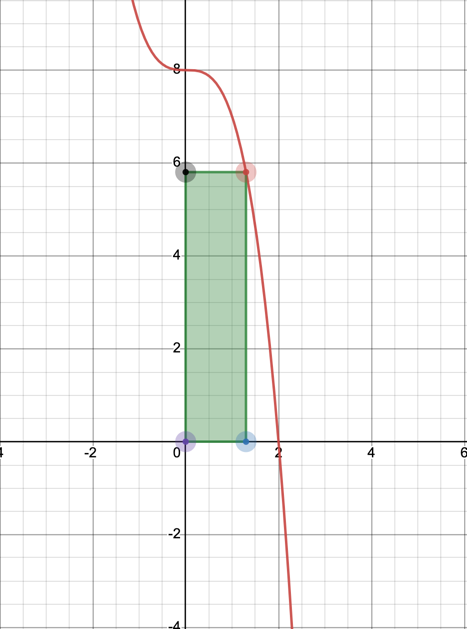
\includegraphics[width=100]{img1}.
    \caption{график функции~\eqref{eq:equation}}
    \label{fig:figure}
\end{figure}

можно увидеть, что в первой четверти графика функция ограничена по оси \(x \in [0,2]\) и \(y \in [0,8]\).

\begin{align}
    S = u \cdot v
    \label{eq:space}
\end{align}

Найдем экстремум функции~\eqref{eq:space}:

\begin{align*}
    v &= -u^3 + 8 \Rightarrow S = u \cdot v = u \cdot (-u^3 + 8) = -u^4+8u \\
    S' &= -4u^3+8 = -4(u^3-2) \Rightarrow u_{max} = 2^{1/3} \Rightarrow v_{max} = -(2^{1/3})^3 + 8 = 6
    \label{eq:equation2}
\end{align*}

Найдём значения площади в граничных значениях и экстремуме:

\begin{align*}
    S_{x=0} &= 0 \\
    S_{x=2} &= 0 \\
    S_{x = u_{max}} &= 6 \cdot 2^{1/3}
    \label{eq:equation3}
\end{align*}

\textbf{Ответ:} \(S_{\max} = 6 \cdot 2^{1/3}, u = 2^{1/3}, v = 6\)
\end{document}